% #############################################################################
% This is Chapter 1
% !TEX root = ../main.tex
% #############################################################################
% Change the Name of the Chapter i the following line
\chapter{Introduction}
% The following line allows to ref this chapter
\label{chap:intro}

The continuous growth and expansion of the world population and the correspondent increase of energy needs, is one of the most relevant topics of the century. The issues caused by the increasing usage of fossil fuels and the amount of carbon dioxide produced everyday is affecting our lives and the future of the planet. In 2019, Industry and buildings account for over 90\% of global electricity demand today, while transport makes up less than 2\% \cite{iea}. Recent studies show that the building sector represents 39\% and 40\% of the energy consumption and 38\% and 36\% of the CO2 emissions in the U.S. \cite{CivilUS} and Europe\cite{CivilEU}, respectively. The expansion of office buildings and the multiplication of the amount of energy needed in order to satisfy the demands of a society that is becoming more and more technologically dependent, are two catalysts for the recent increase of energy consumption. 



On the other hand, sustainable alternatives have also emerged to replace some less ecological social habits. Electric cars are the best example of this. The adoption of electric cars is a practice that has been increasing in the last decade and is expected to grow even more in the next two. Currently the major limitation is the autonomy of the cars, since the batteries still do not have, in most cases, enough capacity to equal the autonomy performance of a fuel car. In this sense, a solution that has been adopted is the installation of charging stations in both residential and office buildings. According to \cite{charger}, the infrastructure for \ac{EV} charging is expanding and in 2019, there were about 7.3 million chargers worldwide, of which about 6.5 million were private. The power spent on charging electric cars in buildings is a new factor to be studied, both in the influence it has on the energy consumption of the building and the reduction of energy waste while using it.


The extent of available data is also multiplying, and the analysis and modeling of this data is becoming essential to minimize energy waste. Modern infrastructures are already equipped with systems able to monitor and control power usage, and there has been an increase in the number of chargers for electric cars installed in garages. The technology also evolved to allow buildings to produce their own energy. The implementation of \ac{PV} panels in buildings is an increasingly common practice. Despite the low efficiencies (from 15\% to 17\% \cite{pv}), \ac{PV} panels are becoming an important energy source for buildings, both  residential and non-residential. 

Modeling energy consumption behaviour and identifying patterns can be crucial both to minimize power usage, and to develop new methodologies to optimize resources. Figure \ref{consumption} illustrates the energy consumption profile of \ac{EDP}'s building in Lisbon, Portugal, between January 25, 2020 and March 13, 2020. The profile illustrated in Figure \ref{consumption} shows a movement that one can identify as a trend. The data presented provides power consumption details for 7 weeks and 7 weekends. The behaviour of the profile tends to be cyclical with a 7 day period. In Figure \ref{production}, one may see the power production profile for the same building and time-interval as Figure \ref{consumption}. The \ac{PV} production behaviour is also cyclical but presents a daily period due to the fact that solar radiation is not influenced by the occupancy rate of the building, so it has no direct relation with the day of the week, but with the hour of the day instead.



\begin{figure}[h!]
\captionsetup[subfigure]{position=b}
\centering
\subcaptionbox{\label{consumption}}{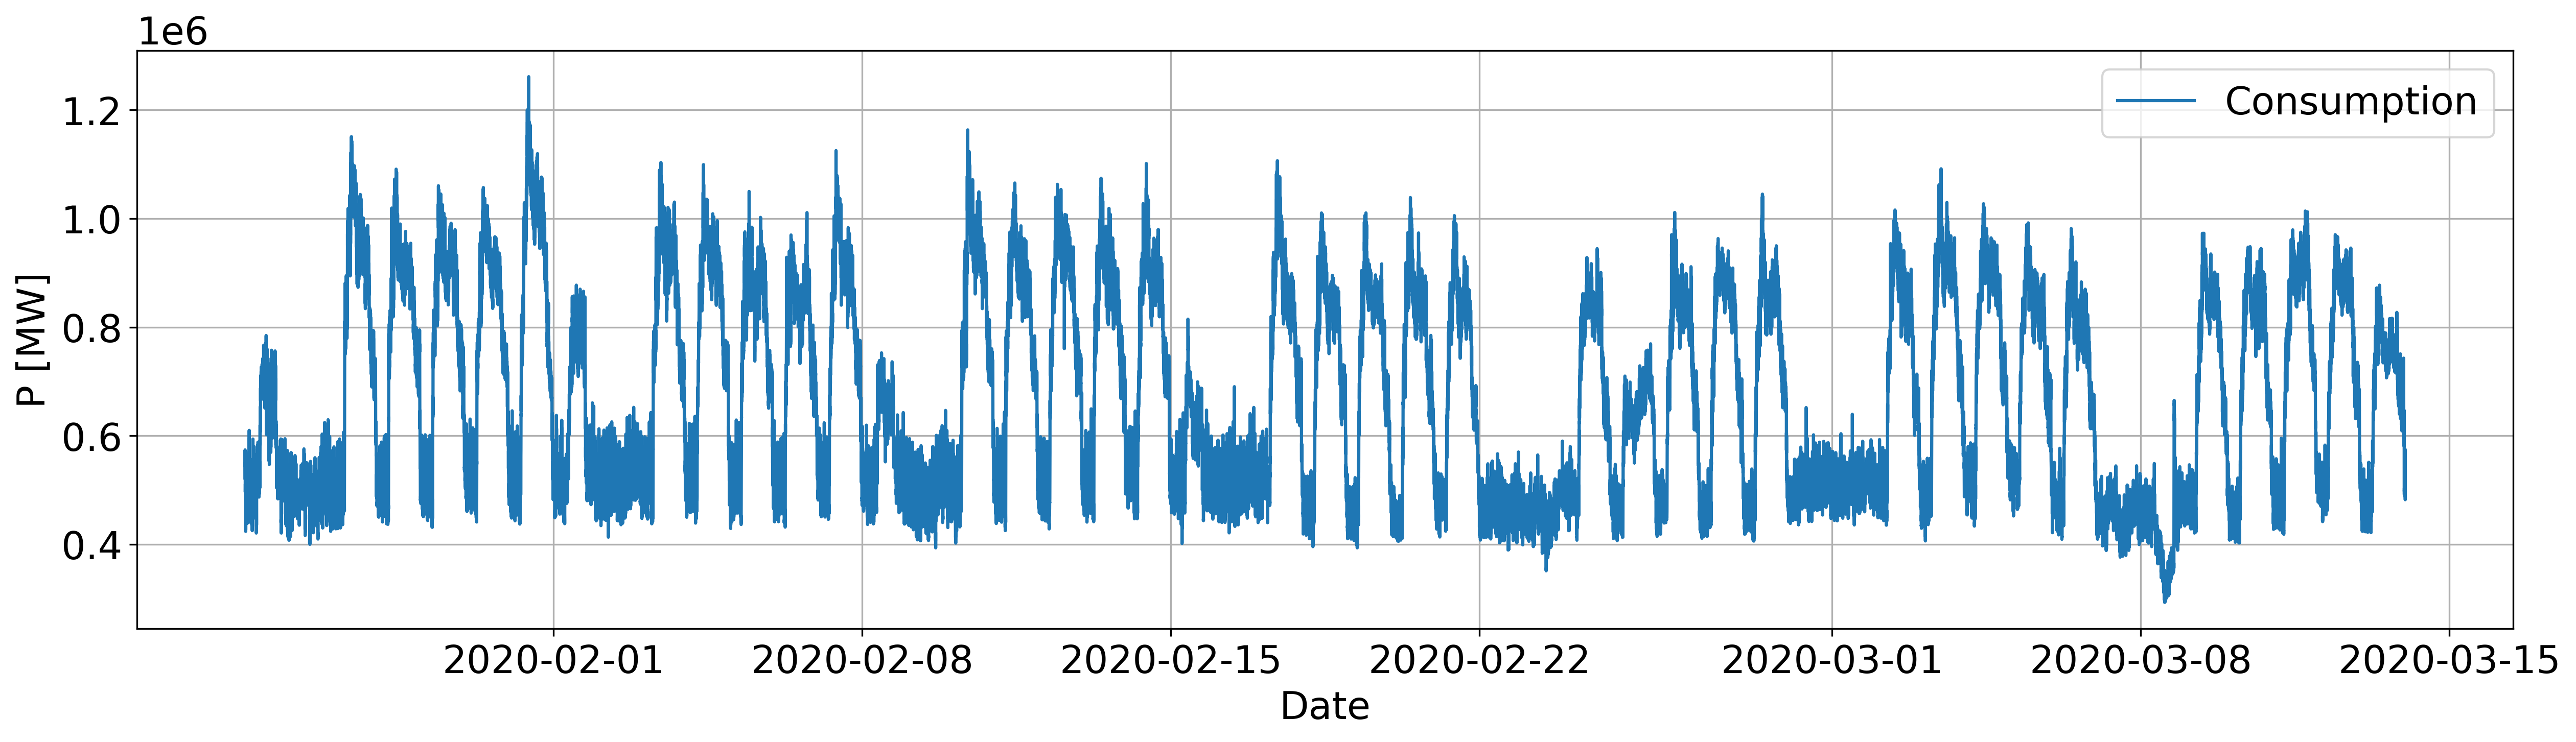
\includegraphics[width=0.9\linewidth]{Images/Consumption_Trend.png}}
\hspace{0.05\textwidth}
\subcaptionbox{ \label{production}}{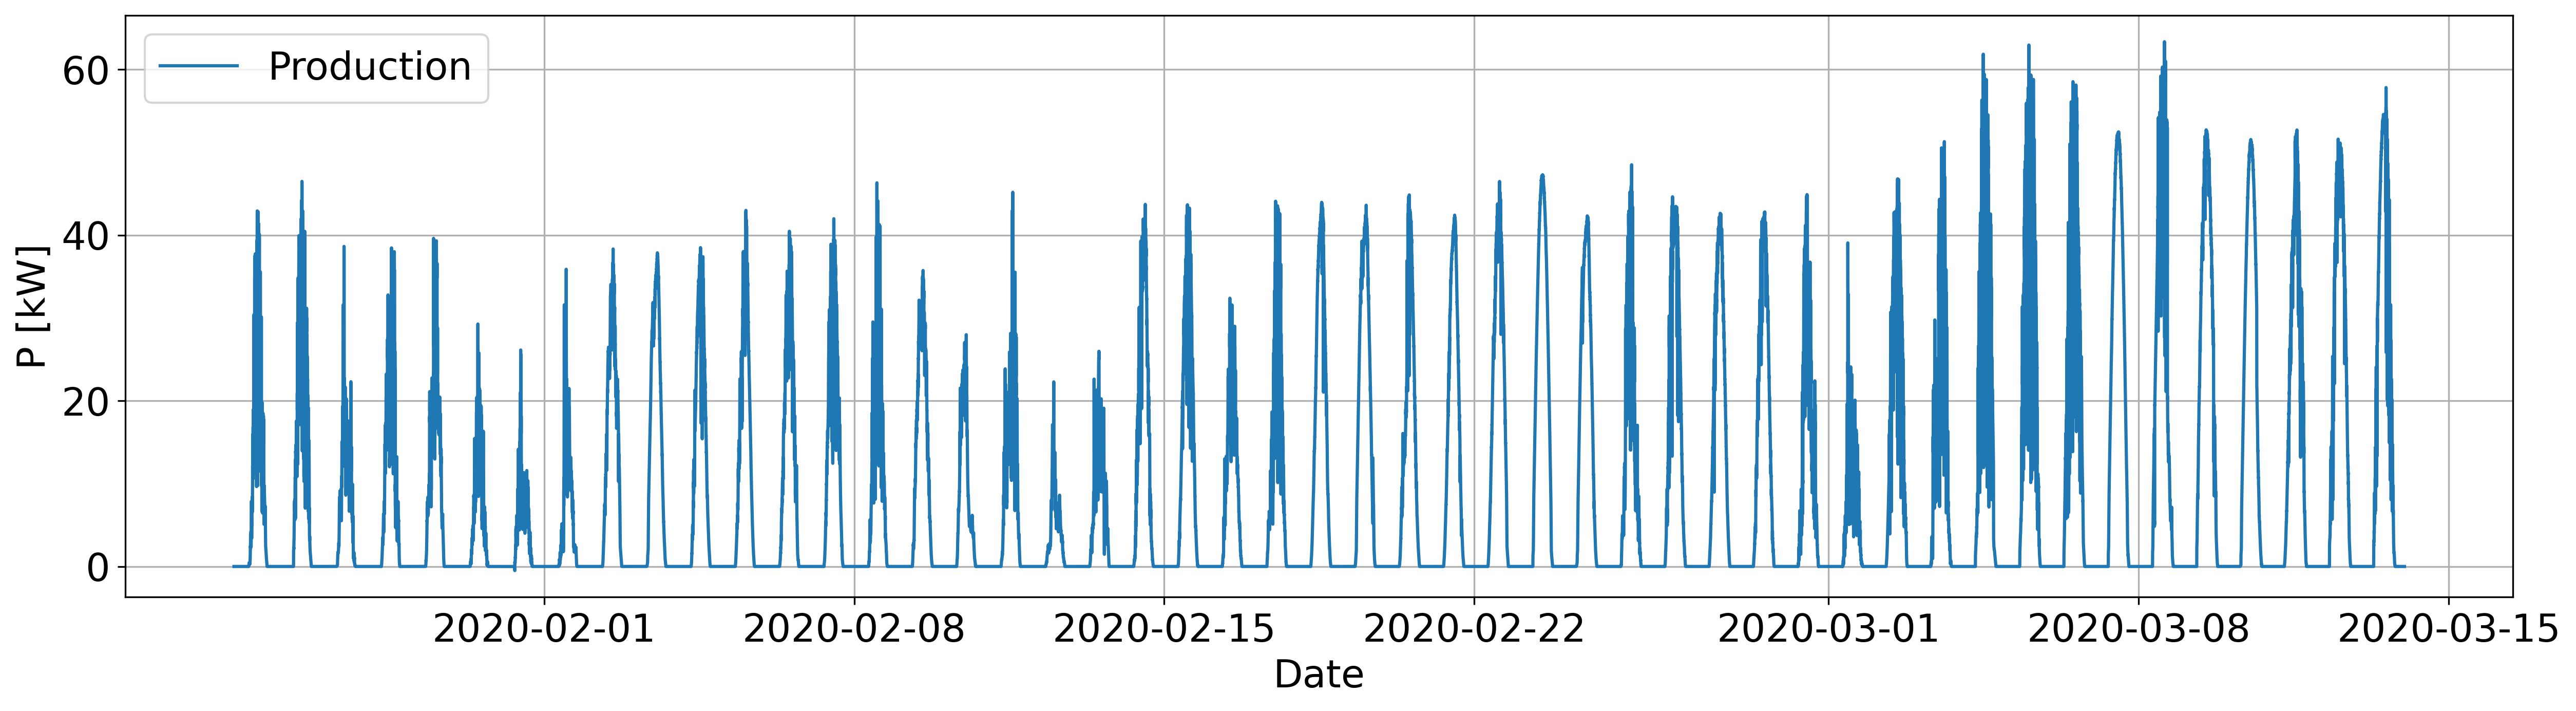
\includegraphics[width=0.9\linewidth]{Images/Production_Trend.png}}
\caption{EDP's building's a) consumption and b) production trends.}
\end{figure}


Variables that present a trend are more easily examined since it is sometimes possible to associate a cause with their cyclical behavior. By identifying this cause, it becomes not only easier to control its current behavior, but also to predict its future behavior. Power consumption forecasting for buildings is a well know area of research. According to \cite{CivilEU}, Energy consumption forecasting plays a significant role in plans to improve energy performance, save energy and reduce the hazardous environmental impact. Moreover, forecasting also plays a vital role in decision-making and future planning which rely on accurate forecasting results. The ability to predict the available power of any building has many interesting utilities. Both power consumption and power production are vital information to have in order to predict power available at each time in the building. With this information, there are multiple innovative ideas that can be implemented with the goal of having a more sustainable and power-optimized building.



\section{Problem statement and objectives}


\ac{EDP} is a vertically integrated energy company with a consolidated position in the Iberian Peninsula, both in terms of electricity generation, distribution and supply, and gas supply. The energy consumption of \ac{EDP}'s Lisbon building can be divided into two categories, controlled and uncontrolled consumption. Within the category of uncontrolled consumption, some factors are identified such as the \ac{HVAC} system, lighting, among others. These factors are said to be uncontrolled, as they generally depend directly on factors such as the outside temperature and the occupancy rate of the building, respectively, variables that cannot be controlled. When it comes to controlled consumption, in the building's parking garage there is an electric car charging system for employees, denominated \ac{EVSCS}. The main functionality of this system is to manage the charging of all the \ac{EV}s connected to the \ac{EVSCSs}. This system is able to assign exactly the amount of power supplied to each vehicle, and is able to prioritize the charging, for example, a vehicle that already has 80$\%$ of battery capacity, has less priority than a discharged vehicle that has been recently connected to the grid. The system can also manage the charging procedure based on the instantaneous available power of the building, providing more capacity when there is less overall consumption, and reducing the capacity otherwise. The decision making ability of the \ac{EVSCS} makes the charging of \ac{EV}s a controlled consumption process. When it comes to production, unlike generality, the building is equipped with 70 kWp (kilowatt "peak") of solar generation, which means it also has the capacity to generate power. 


%The ability to forecast building power consumption's and the respective power available at each time, can be decisive to optimize power usage in a building.  


%Regarding energy profile, there are two main types of buildings, residential buildings and non-residential buildings. A building should be regarded as residential building when more than half of the floor area is used for dwelling purposes \cite{OECD}. On the other hand, non-residential buildings consists of buildings other than dwellings, including fixtures, facilities and equipment that are integral parts of the structures and costs of site clearance and preparation \cite{OECD}. The work presented focuses on non-residential buildings, more specifically office buildings.

 
Taking into consideration the listed factors, the work developed in this thesis contributes directly to minimize the unnecessary power consumption, thus contributing to a more sustainable building. At a global scale, the objective is to assist \ac{EVSCS} in the handling of power utilization in the  \ac{EV}'s charging procedure. The system has access to current data, namely the total power available at each instant, but it would be useful to obtain a forecast of the power available in the near future. The knowledge of this value would bring enormous advantages, positively impacting the way \ac{EV} charging is managed. The question then arises: "How can one forecast the power available in a near future, in order to optimize the \ac{EVSCS}?


To answer this question, it is then considered that the specific goal is to create a computing architecture capable of predicting the energy available in the future, while using that forecast to feed the \ac{EVSCS}. Specifically, the goal is to define a short-term power availability forecast system to help the \ac{EVSCS} to manage power supply for \ac{EVSCSs}.

The expected result of the research should be (but not limited to) a maximum and minimum power output forecast algorithm to boost the capabilities of the \ac{EVSCS} by predicting \ac{EDP}'s building power availability for the next 5, 10 and/or 15 minutes:
\begin{enumerate}[noitemsep,topsep=0pt]
  \itemsep0em 
  \item Make predictions and compare the results for different time-frames (5, 10 and 15 minutes);
  \item Serve the power demand prediction outputs as inputs for a decision-based algorithm to act directly on the “\ac{EV} Smart Charging” Stations.
\end{enumerate}   



\section{Thesis outcome}


In the course of this dissertation, a predictive model based on \ac{ML} methodologies was developed, namely using \ac{ANN}s, capable of producing forecasts of the available power with a time target of 5, 10 and 15 minutes in the future, for a building that presents two peculiar characteristics: it has panels \ac{PV} for energy production and it has an electric car loading system in its parking garage. Eight different types of architectures were tested and their performance was studied for specific cases. The result is an automated predictive system that uses XXXXX.

In the process of carrying out this research, meteorological and radiation data provided by \ac{FCUL} were used, as well as data regarding the energy production and consumption of the building, provided by \ac{EDP}.

The work carried out followed the following steps:
\begin{enumerate}[noitemsep,topsep=0pt]
  \itemsep0em 
  \item Data cleaning;
  \item Data prepossessing;
  \item Comparison between eight predictive architectures.
  \item Selection of the best predictive architectures.
  \item Selection of the final architectures for specific scenarios.
  \item Construction of an automated forecasting system.
\end{enumerate}


In Figure \ref{scope} it is possible to observe a diagram of the total architecture of the work developed in this thesis. 

\begin{figure}[h!]
    \centering
    \begin{center}
    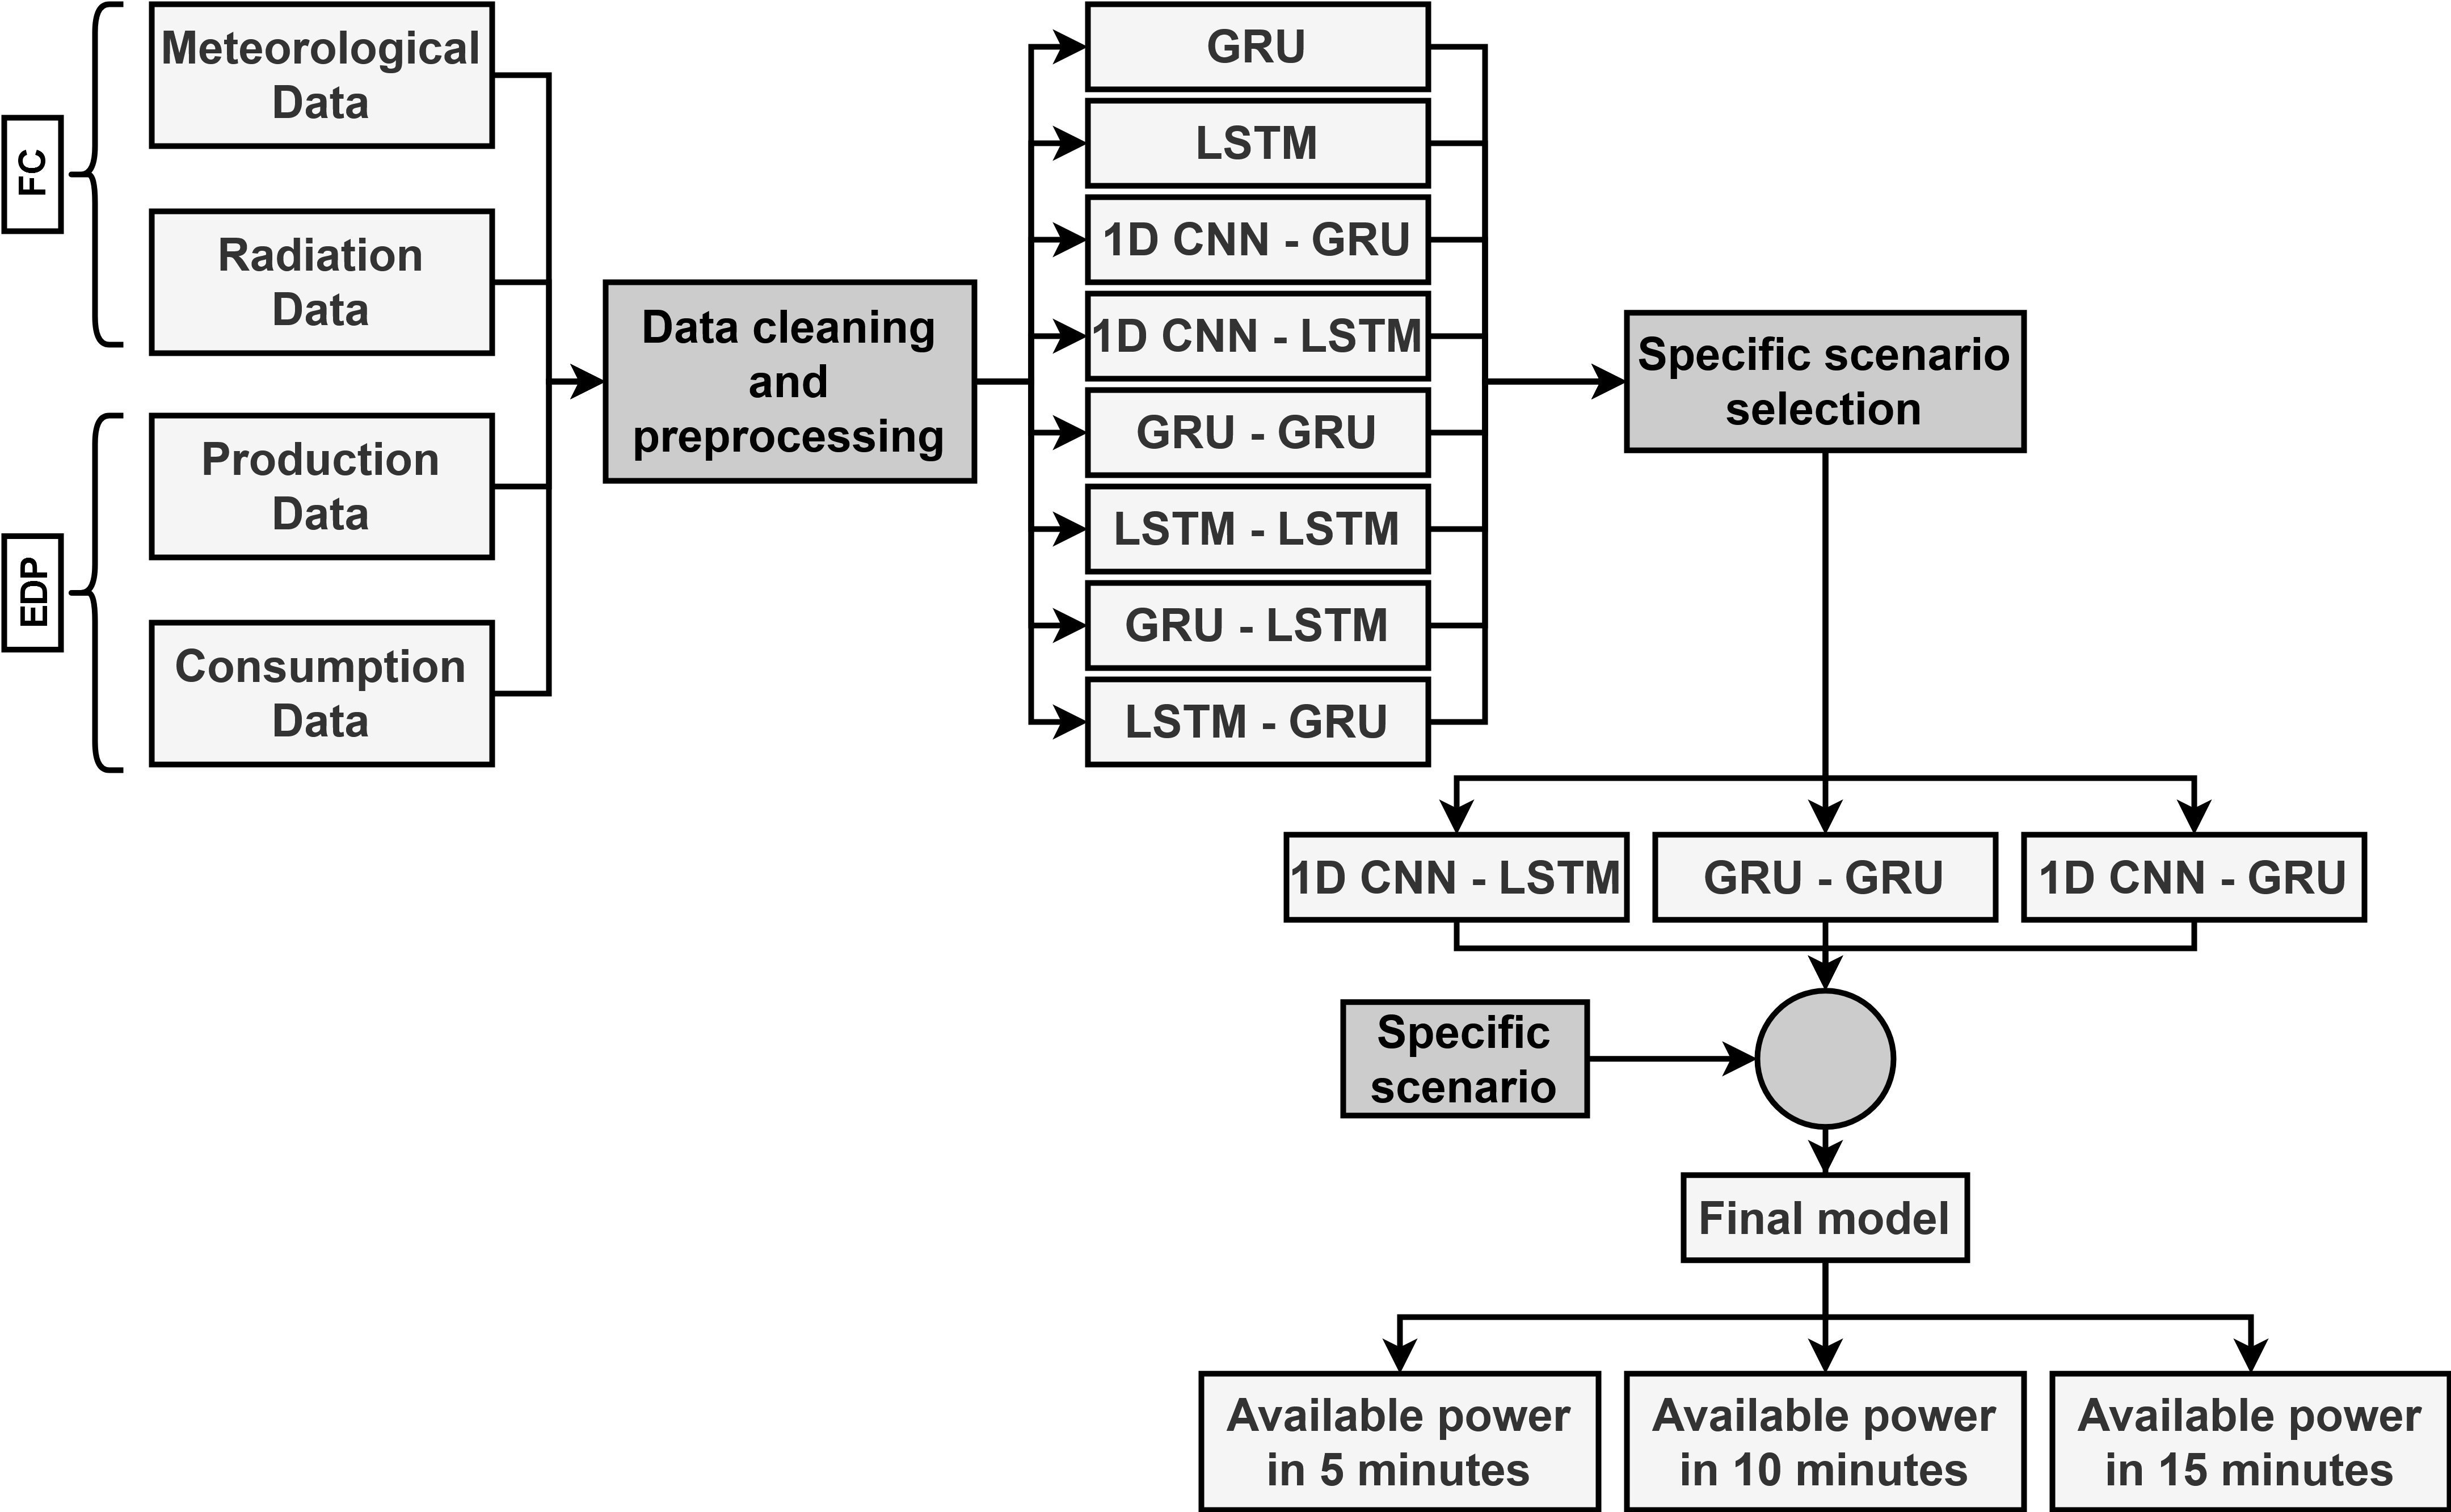
\includegraphics[width=1\textwidth]{Images/Work.png}
    \caption{Thesis framework.}
    \label{scope}
    \end{center}
\end{figure}

The purpose of this thesis is to implement a system capable of computing the available power in the near future. A total of four datesets were used, with information on solar radiation, the weather conditions of the area where the building is located, the consumption and production of the building. These data, besides having different dimensions and granularities, presented temporal gaps. It was then necessary to automate a data treatment process in which, regardless of the state in which the data are introduced in the system, they are treated and prepared to respect the structure that allows them to be used as inputs to the system. At a later stage, eight different \ac{ANN} architectures composed of three categories of distinct layers were designed: \ac{GRU}, \ac{LSTM} and \ac{1D CNN}. After performing some tests, the three final models were then chosen that present the best performance for three distinct situations: weekdays, weekends and holidays. The last step was to build a system capable of choosing the model to be used based on the situation you want to foresee. It was then arrived to a system capable of performing, with minimum error, the forecast of the total power available in the building in 5, 10 and 15 minutes. These data are later provided to the \ac{EVSCS} that will use them to optimize its decision process. The optimization process of the charging system is outside the scope of this thesis.





\section{Thesis outline}